\documentclass[a4paper,11pt,titlepage]{jarticle}
\usepackage[dvipdfmx]{graphicx}
\usepackage{listings}
\usepackage{amsmath}
\usepackage{fancybox,ascmac}
\usepackage{url}

\title{知能情報実験II(第8回):「無線通信における降水減衰特性のモデリング」}
\author{175751C 宮城孝明}
\date{\today}
\begin{document}
\maketitle
\tableofcontents
\clearpage

\section{実験の目的}

衛星通信や FWA(Fixed Wireless Access:固定無線通信)といった、10GHz を超える ような周波数帯を用いた無線通信では、降雨現象が大きな問題となる事が知られている。 とりわけ、沖縄県のような亜熱帯地方に属する気候区では、スコールと呼ばれる大雨や台 風による豪雨など、年間を通して頻繁に発生する。そのような地方で安定した無線通信を 行うには、降雨による電波の減衰(降雨減衰と呼びます)を定量的に把握し、それに対処 する必要がある。つまり、降雨減衰特性をモデリングすることが必須になる。 本実験では、本学 1 号館の屋上に設置された FWA(18GHz帯、26GHz帯)の受信 レベルと降雨強度(1 分間の降雨量)の 3 つのデータを用いて、琉球大学周辺における18 GHz帯、26GHz帯の無線通信における降雨減衰特性のモデリングを行う。なお、今回 用いるデータはここだけにしか存在しない学術的に貴重なもの(研究論文のネタになる!) であり、宮里研究室の卒業研究テーマの一つに活用されている。本実験を通して、卒業研 究の入り口を体験してみよう。
\section{実験の概要}
実験中に与えられたデータをもとに,手順1から7を通し,データを加工する.加工したデータを可視化し易いようにグラフにして示す.

\section{実験の結果}

\subsection{10sずつの変換と物理量の変換}
\subsubsection{18GHzコード}
\lstinputlisting[language=python, numbers=left, breaklines=true, basicstyle=\ttfamily\footnotesize,
  frame=single, caption=Rx18GHz\_data, label=sample]{Rx18_data.py}

\subsubsection{26GHzコード}
\lstinputlisting[language=python, numbers=left, breaklines=true, basicstyle=\ttfamily\footnotesize,
  frame=single, caption=Rx26GHz\_data, label=sample]{Rx26_data.py}

\subsection{降水強度のデータプログラム}
\subsubsection{降水時間を変換コード}
\lstinputlisting[language=python, numbers=left, breaklines=true, basicstyle=\ttfamily\footnotesize,
  frame=single, caption=Rain\_data, label=sample]{rain_data.py}

\subsubsection{降水間隔}
RainDataの最大値が150mm/h : 5mmとする\par
Rx18GHzの最大値が-25mm/h : -3mmとする\par
Rx26GHzの最大値が-10mm/h : -3mmとする\par

\subsubsection{コード}
\lstinputlisting[language=python, numbers=left, breaklines=true, basicstyle=\ttfamily\footnotesize,
  frame=single, caption=Rain\_result, label=sample]{Rain_ac.py}

\lstinputlisting[language=python, numbers=left, breaklines=true, basicstyle=\ttfamily\footnotesize,
  frame=single, caption=Rx18GHz\_result, label=sample]{Rx18_result.py}

\lstinputlisting[language=python, numbers=left, breaklines=true, basicstyle=\ttfamily\footnotesize,
  frame=single, caption=Rx26GHz\_result, label=sample]{Rx26_result.py}
\subsection{グラフ}
\subsubsection{コード}
\lstinputlisting[language=python, numbers=left, breaklines=true, basicstyle=\ttfamily\footnotesize,
  frame=single, caption=Rain\_grahp, label=sample]{Rain_graph.py}
\lstinputlisting[language=python, numbers=left, breaklines=true, basicstyle=\ttfamily\footnotesize,
  frame=single, caption=Rx18\_graph, label=sample]{Rx18_graph.py}
\lstinputlisting[language=python, numbers=left, breaklines=true, basicstyle=\ttfamily\footnotesize,
  frame=single, caption=Rx26GHz\_graph, label=sample]{Rx26_graph.py}
\subsubsection{出力}
\begin{figure}[htbp]
  \centering
  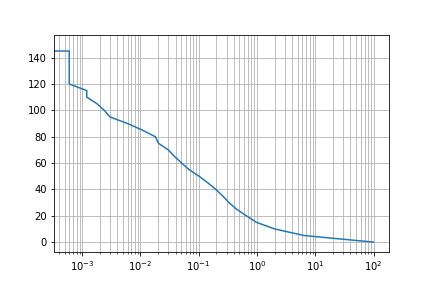
\includegraphics[width=80mm]{Rain_cd.png}
  \label{Rainデータの累積分布図}\\
  \caption{Rainデータの累積分布図}
\end{figure}

\begin{figure}[htbp]
  \centering
  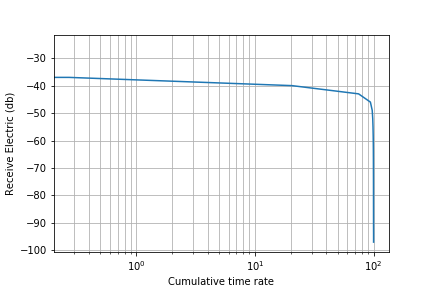
\includegraphics[width=80mm]{Rx18_cd.png}
  \label{Rx18の累積分布図}\\
  \caption{Rx18の累積分布図}
\end{figure}

\begin{figure}[htbp]
  \centering
  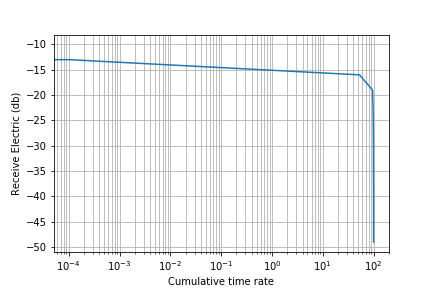
\includegraphics[width=80mm]{Rx26_cd.png}
  \label{Rx26の累積分布図}\\
  \caption{Rx26の累積分布図}
\end{figure}

\clearpage

\section{考察}
Rainの累積分布は,100(mm/h)を超える確率は,100分の1以下程度であるとわかる.つまり,1年に1時間程度しか100mm/hの雨が降らないことがこのグラフからわかる.\par
結果から見ると,降雨強度が高ければ,受信電界が低なる.つまり,降雨量が上がれば電波通信に影響が起きることがわかる.
Rx18GHzとRx26GHzの累積分布図を見てみる.一見どちらも似たようなグラフになっているが,Rx26GHzの方が累積時間率が細かくなっている.さらに,受信電界も最大値は
Rx26GHzが高い.つまり,Rx26GHzの方がRx18GHzより降雨量の影響が受けないと予想される.




\end{document}
